
% LaTeX Beamer file automatically generated from DocOnce
% https://github.com/doconce/doconce

%-------------------- begin beamer-specific preamble ----------------------

\documentclass{beamer}

\usetheme{red_plain}
\usecolortheme{default}

% turn off the almost invisible, yet disturbing, navigation symbols:
\setbeamertemplate{navigation symbols}{}

% Examples on customization:
%\usecolortheme[named=RawSienna]{structure}
%\usetheme[height=7mm]{Rochester}
%\setbeamerfont{frametitle}{family=\rmfamily,shape=\itshape}
%\setbeamertemplate{items}[ball]
%\setbeamertemplate{blocks}[rounded][shadow=true]
%\useoutertheme{infolines}
%
%\usefonttheme{}
%\useinntertheme{}
%
%\setbeameroption{show notes}
%\setbeameroption{show notes on second screen=right}

% fine for B/W printing:
%\usecolortheme{seahorse}

\usepackage{pgf}
\usepackage{graphicx}
\usepackage{epsfig}
\usepackage{relsize}

\usepackage{fancybox}  % make sure fancybox is loaded before fancyvrb

\usepackage{fancyvrb}
\usepackage{minted} % requires pygments and latex -shell-escape filename
%\usepackage{anslistings}
%\usepackage{listingsutf8}

\usepackage{amsmath,amssymb,bm}
%\usepackage[latin1]{inputenc}
\usepackage[T1]{fontenc}
\usepackage[utf8]{inputenc}
\usepackage{colortbl}
\usepackage[english]{babel}
\usepackage{tikz}
\usepackage{framed}
% Use some nice templates
\beamertemplatetransparentcovereddynamic

% --- begin table of contents based on sections ---
% Delete this, if you do not want the table of contents to pop up at
% the beginning of each section:
% (Only section headings can enter the table of contents in Beamer
% slides generated from DocOnce source, while subsections are used
% for the title in ordinary slides.)
\AtBeginSection[]
{
  \begin{frame}<beamer>[plain]
  \frametitle{}
  %\frametitle{Outline}
  \tableofcontents[currentsection]
  \end{frame}
}
% --- end table of contents based on sections ---

% If you wish to uncover everything in a step-wise fashion, uncomment
% the following command:

%\beamerdefaultoverlayspecification{<+->}

\newcommand{\shortinlinecomment}[3]{\note{\textbf{#1}: #2}}
\newcommand{\longinlinecomment}[3]{\shortinlinecomment{#1}{#2}{#3}}

\definecolor{linkcolor}{rgb}{0,0,0.4}
\hypersetup{
    colorlinks=true,
    linkcolor=linkcolor,
    urlcolor=linkcolor,
    pdfmenubar=true,
    pdftoolbar=true,
    bookmarksdepth=3
    }
\setlength{\parskip}{0pt}  % {1em}

\newenvironment{doconceexercise}{}{}
\newcounter{doconceexercisecounter}
\newenvironment{doconce:movie}{}{}
\newcounter{doconce:movie:counter}

\newcommand{\subex}[1]{\noindent\textbf{#1}}  % for subexercises: a), b), etc

%-------------------- end beamer-specific preamble ----------------------

% Add user's preamble




% insert custom LaTeX commands...

\raggedbottom
\makeindex

%-------------------- end preamble ----------------------

\begin{document}

% matching end for #ifdef PREAMBLE

\newcommand{\exercisesection}[1]{\subsection*{#1}}



% ------------------- main content ----------------------



% ----------------- title -------------------------

\title{Basic elements of quantum computing}

% ----------------- author(s) -------------------------

\author{Nuclear TALENT course on quantum computing\inst{}}
\institute{}
% ----------------- end author(s) -------------------------

\date{Monday June 23, 2025
% <optional titlepage figure>
% <optional copyright>
}

\begin{frame}[plain,fragile]
\titlepage
\end{frame}

\begin{frame}[plain,fragile]
\frametitle{Overview of Monday June 23 and plans for the second week}

\begin{block}{}
\begin{enumerate}
\item Simple Hamiltonian matrices, one and two-qubit examples

\item Introducing the Variational Quantum Eigensolver algorithm

\item Parametrized quantum circuits

\item Introducing the Lipkin model (nuclear structure classic)

\item Tuesday to Friday we plan to discuss more realistic nuclear physics Hamiltonians, the  Jordan-Wigner transformation, time evolution, Quantum Fourier transforms, Quantum Phase estimation, quantum state preparation, quantum error propagation and more
\end{enumerate}

\noindent
\end{block}
\end{frame}

\begin{frame}[plain,fragile]
\frametitle{Hamiltonians, one-qubit example}

As an initial test, we consider a simply $2\times 2$ real
Hamiltonian consistend of a diagonal part $H_0$ and off-diagonal part
$H_I$, playing the roles of a non-interactive one-body and interactive
two-body part respectively. Defined through their matrix elements, we
express them in the Pauli basis $\vert 0\rangle$ and $\vert 1 \rangle$

\begin{align*}
    \begin{split} 
        H &= H_0 + H_I \\
        H_0 = \begin{bmatrix}
            E_1 & 0 \\
            0 & E_2
        \end{bmatrix}&, \hspace{20px}
        H_I = \lambda \begin{bmatrix}
            V_{11} & V_{12} \\
            V_{21} & V_{22}
        \end{bmatrix}
    \end{split}
\end{align*}
Where $\lambda \in [0,1]$ is a coupling constant parameterizing the strength of the interaction.
\end{frame}

\begin{frame}[plain,fragile]
\frametitle{Rewriting in terms of Pauli matrices}

Defining
\[
    E_+ = \frac{E_1 + E_2}{2},\hspace{20px} E_- = \frac{E_1 - E_2}{2}
\]
we see that by combining the identity and $Z$ Pauli matrix, this can be expressed as

\[
    H_0 = E_+ I + E_- Z
\]

For $H_1$ we use the same trick to fill the diagonal, defining $V_+ = (V_{11} + V_{22})/2, V_- = (V_{11} - V_{22})/2$. From the hermiticity requirements of $H$, we note that $V_{12} = V_{21} \equiv V_o$, which simplifies the problem to a simple $X$. This gives

\[
    H_I = V_+ I + V_- Z + V_o X
\]
\end{frame}

\begin{frame}[plain,fragile]
\frametitle{Measurement basis}

For this system we note that the Pauli $X$ matrix can be rewritten in terms of the Hadamard matrices and the Pauli $Z$ matrix (exercises from Monday-Tuesday of week 1), that is
\[
X=HZH.
\]
\end{frame}

\begin{frame}[plain,fragile]
\frametitle{Second Hamiltonian matrix problems, two-qubit case}

The second case is defined as a $4 \times 4$ real Hamiltonian.
This can be viewed as two  composite systems where each system is represented by a two-level system. In the product basis $\vert 00\rangle$, $\vert 01\rangle$, $\vert 10\rangle$ and $\vert 11\rangle$ (our computational basis)
we define the one-body part as 
\[
    H_0 \vert ij \rangle = \epsilon_{ij}\vert ij\rangle, 
\]
with a two-body interaction defined as

\begin{align*}
    \begin{split} 
        H_I &= H_x X \otimes X + H_z Z \otimes Z \\
        &= \begin{bmatrix}
            H_z & 0 & 0 & H_z \\
            0 & - H_z & H_x & 0 \\
            0 & H_x & - H_z & 0 \\
            H_x & 0 & 0 & H_z
        \end{bmatrix}.
    \end{split}
\end{align*}

Here $H_x$ and $H_z$ are coupling constants.
\end{frame}

\begin{frame}[plain,fragile]
\frametitle{Rewriting}

For the $4 \times 4$ case, the interacting part of the
Hamiltonian is already
written in terms of Pauli matrices. On the other hand, we need to rewrite the diagonal term.
We define
\begin{align*}
    \epsilon_{\pm 0} = \frac{\epsilon_{00}\pm\epsilon_{01}}{2},\hspace{20px}\epsilon_{\pm 1} = \frac{\epsilon_{10}\pm\epsilon_{11}}{2}.
\end{align*}
We note that the energies $\epsilon_{00}$ and $\epsilon_{01}$ can be repeated on the diagonal. This is also the case for $\epsilon_{10}$ and $\epsilon_{11}$
\begin{align*}
    D_{0} &= \epsilon_{+0} I\otimes I + \epsilon_{-0} I\otimes Z, \\
    D_{1} &= \epsilon_{+0} I\otimes I + \epsilon_{-1} I\otimes Z.
\end{align*}
\end{frame}

\begin{frame}[plain,fragile]
\frametitle{Further manipulations}

Using the Pauli $Z$ matrix and the identity matrix $I$ we define
\begin{align*}
    P_{\pm} = \frac{1}{2}(I \pm Z),
\end{align*}
which we use to project out the first and last to two elements the of $4\times 4$ matrix
\[
    P_0 = P_+ \otimes I,\hspace{20px}P_0 = P_- \otimes I.
\]
Adding $D_0$ and $D_1$, we get
\[
    H_0 = P_0 D_0 + P_1 D_1= \alpha_+ I \otimes I + \alpha_- Z \otimes I + \beta_+ I \otimes Z + \beta_- Z \otimes Z, 
\]
where we have defined
\[
    \alpha_\pm = \frac{\epsilon_{+0}\pm\epsilon_{+1}}{2}, \hspace{10px} \beta_\pm = \frac{\epsilon_{-0}\pm\epsilon_{+1}}{2}
\]
\end{frame}

\begin{frame}[plain,fragile]
\frametitle{The Lipkin model, more details below}

For the Lipkin model, we recommend strongly the work of LaRose and collaborators, see
\href{{https://journals.aps.org/prc/abstract/10.1103/PhysRevC.106.024319}}{\nolinkurl{https://journals.aps.org/prc/abstract/10.1103/PhysRevC.106.024319}}, see in particular section 3.

For codes, feel free to be inspired and/or reuse the codes at \href{{https://github.com/CompPhysics/QuantumComputingMachineLearning/tree/gh-pages/doc/Programs/LipkinModel}}{\nolinkurl{https://github.com/CompPhysics/QuantumComputingMachineLearning/tree/gh-pages/doc/Programs/LipkinModel}}.
\end{frame}

\begin{frame}[plain,fragile]
\frametitle{States, gates and measurements, reminder from last week}

Mathematically, quantum gates are a series of unitary operators in the
operator space defined by our Hamiltonian $\mathcal{H}$ and operators $\mathcal{O}$ which evolve a given initial
state. The unitary nature preserves the norm of the state vector,
ensuring the probabilities sum to unity. Since not all gates
correspond to an observable, they are not all necessarily hermitian.
\end{frame}

\begin{frame}[plain,fragile]
\frametitle{Single qubit gates}

The Pauli matrices (and gate operations following therefrom) are defined as
\[
	\bm{X} \equiv \sigma_x = \begin{bmatrix}
		0 & 1 \\
		1 & 0
	\end{bmatrix}, \quad
	\bm{Y} \equiv \sigma_y = \begin{bmatrix}
		0 & -i \\
		i & 0
	\end{bmatrix}, \quad
	\bm{Z} \equiv \sigma_z = \begin{bmatrix}
		1 & 0 \\
		0 & -1
	\end{bmatrix}.
\]
\end{frame}

\begin{frame}[plain,fragile]
\frametitle{Pauli-${\bf X}$ gate}

The Pauli-$\bm{X}$ gate is also known as the \textbf{NOT} gate, which flips the state of the qubit.
\begin{align*}
	\bm{X}\vert 0\rangle &= \vert 1\rangle, \\
	\bm{X}\vert 1\rangle &= \vert 0\rangle.	
\end{align*}
The Pauli-$\bm{Y}$ gate flips the bit and multiplies the phase by $ i $. 
\begin{align*}
	\bm{Y}\vert 0\rangle &= i\vert 1\rangle, \\
	\bm{Y}\vert 1\rangle &= -i\vert 0\rangle.
\end{align*}
The Pauli-$\bm{Z}$ gate multiplies only the phase of $\vert 1\rangle$ by $ -1 $.
\begin{align*}
	\bm{Z}\vert 0\rangle &= \vert 0\rangle, \\
	\bm{Z}\vert 1\rangle &= -\vert 1\rangle.
\end{align*}
\end{frame}

\begin{frame}[plain,fragile]
\frametitle{Hadamard gate}

The Hadamard gate is defined as
\[
	\bm{H} = \frac{1}{\sqrt{2}} \begin{bmatrix}
		1 & 1 \\
		1 & -1
	\end{bmatrix}.
\]

It creates a superposition of the $ \vert 0\rangle $ and $ \vert 1\rangle $ states.
\begin{align}
	\bm{H}\vert 0\rangle &= \frac{1}{\sqrt{2}} \left( \vert 0\rangle + \vert 1\rangle \right), \\
	\bm{H}\vert 1\rangle &= \frac{1}{\sqrt{2}} \left( \vert 0\rangle - \vert 1\rangle \right).
\end{align}
Note that we will use $H$ as symbol for the Hadamard gate while we will reserve the notation $\mathcal{H}$ for a given Hamiltonian.
\end{frame}

\begin{frame}[plain,fragile]
\frametitle{Phase Gates}

The phase gate is usually denoted as $S$ and is defined as
\[
	\bm{S} = \begin{bmatrix}
		1 & 0 \\
		0 & i
	\end{bmatrix}.
\]
It multiplies only the phase of the $ \vert 1\rangle $ state by $ i $.
\begin{align*}
	\bm{S}\vert 0\rangle &= \vert 0\rangle, \\
	\bm{S}\vert 1\rangle &= i\vert 1\rangle.
\end{align*}
\end{frame}

\begin{frame}[plain,fragile]
\frametitle{The  inverse of the $\bm{S}$-gate}

The inverse
\[
	\bm{S}^\dagger = \begin{bmatrix}
		1 & 0 \\
		0 & -i
	\end{bmatrix}
\]
is known as the $ \bm{S}^\dagger$ gate which applies an $\imath$ phase shift to $\vert 1\rangle$.
\begin{align*}
	\bm{S}^\dagger\vert 0\rangle &= \vert 0\rangle, \\
	\bm{S}^\dagger\vert 1\rangle &= -i\vert 1\rangle.
\end{align*}
\end{frame}

\begin{frame}[plain,fragile]
\frametitle{Two-qubit gates}

The CNOT gate is a two-qubit gate which acts on two qubits, a control qubit and a target qubit. The CNOT gate is defined as
\[
	\text{CNOT} = \begin{bmatrix}
		1 & 0 & 0 & 0 \\
		0 & 1 & 0 & 0 \\
		0 & 0 & 0 & 1 \\
		0 & 0 & 1 & 0
	\end{bmatrix}.
\]
It is often used to perform linear entanglement on qubits.
\begin{align*}
	\text{CNOT} \vert 00\rangle &= \vert 00\rangle, \\
	\text{CNOT} \vert 01\rangle &= \vert 01\rangle, \\
	\text{CNOT} \vert 10\rangle &= \vert 11\rangle, \\
	\text{CNOT} \vert 11\rangle &= \vert 10\rangle.
\end{align*}
\end{frame}

\begin{frame}[plain,fragile]
\frametitle{The SWAP gate}

The SWAP gate is a two-qubit gate which swaps the state of two qubits. It is defined as
\[
	\text{SWAP} = \begin{bmatrix}
		1 & 0 & 0 & 0 \\
		0 & 0 & 1 & 0 \\
		0 & 1 & 0 & 0 \\
		0 & 0 & 0 & 1
	\end{bmatrix}.
\]
\begin{align*}
	\text{SWAP}\vert 00\rangle &= \vert 00\rangle, \\
	\text{SWAP} \vert 01\rangle &= \vert 10\rangle, \\
	\text{SWAP} \vert 10\rangle &= \vert 01\rangle, \\
	\text{SWAP} \vert 11\rangle &= \vert 11 \rangle.
\end{align*}
\end{frame}

\begin{frame}[plain,fragile]
\frametitle{Pauli Strings}

A Pauli string, such as $\bm{XIYZ}$ is a tensor product of Pauli matrices acting on different qubits.
The Pauli string $\bm{XIYZ}$ is defined as (from qubit one to qubit four, from left to right)
\[
	\bm{XIYZ} \equiv \bm{X}_0 \otimes \bm{I}_1 \otimes \bm{Y}_2 \otimes \bm{Z}_3.
\]
Hamiltonians are often rewritten or decomposed in terms of Pauli string as they can be easily implemented on quantum computers.
\end{frame}

\begin{frame}[plain,fragile]
\frametitle{Variational Quantum Eigensolver}

An important  algorithm to estimate the eigenenergies of a quantum
Hamiltonian is \href{{https://qiskit.org/textbook/ch-algorithms/quantum-phase-estimation.html}}{quantum phase
estimation}. In
it, one encodes the eigenenergies, one binary bit at a time (up to $n$
bits), into the complex phases of the quantum states of the Hilbert
space for $n$ qubits. It does this by applying powers of controlled
unitary evolution operators to a quantum state that can be expanded in
terms of the Hamiltonian's eigenvectors of interest. The eigenenergies
are encoded into the complex phases in such a way that taking the
inverse quantum Fourier transformation (see Hundt sections 6.1-6.2) of
the states into which the eigen-energies are encoded results in a
measurement probability distribution that has peaks around the bit
strings that represent a binary fraction which corresponds to the
eigen-energies of the quantum state acted upon by the controlled
unitary operators. We will discuss the QPE on Wednesday this week.
\end{frame}

\begin{frame}[plain,fragile]
\frametitle{The VQE}

While quantum phase estimation (QPE) is provably efficient,
non-hybrid, and non-variational, the number of qubits and length of
circuits required is too great for our NISQ era quantum
computers. Thus, QPE is only efficiently applicable to large,
fault-tolerant quantum computers that likely won't exist in the near,
but the far future.

Therefore, a different algorithm for finding the eigen-energies of a
quantum Hamiltonian was put forth in 2014 called the variational
quantum eigensolver, commonly referred to as
\href{{https://arxiv.org/abs/2111.05176}}{VQE}. The algorithm is hybrid,
meaning that it requires the use of both a quantum computer and a
classical computer. It is also variational, meaning that it relies,
ultimately, on solving an optimization problem by varying parameters
and thus is not as deterministic as QPE. The variational quantum
eigensolver is based on the variational principle:
\end{frame}

\begin{frame}[plain,fragile]
\frametitle{Rayleigh-Ritz variational principle}

Our starting point is the Rayleigh-Ritz variational principle states
that for a given Hamiltonian $H$, the expectation value of a trial
state or just ansatz $\vert \psi \rangle$ puts a lower bound on the
ground state energy $E_0$.

\[
    \frac{\langle \psi \vert \mathcal{H}\vert \psi \rangle}{\langle \psi \vert \psi \rangle} \geq E_0.
\]
\end{frame}

\begin{frame}[plain,fragile]
\frametitle{The ansatz}

The ansatz is typically chosen to be a parameterized superposition of
basis states that can be varied to improve the energy estimate,
$\vert \psi\rangle \equiv \vert \psi(\boldsymbol{\theta})\rangle$ where
$\boldsymbol{\theta} = (\theta_1, \ldots, \theta_M)$ are the $M$
optimization parameters.
\end{frame}

\begin{frame}[plain,fragile]
\frametitle{Expectation value of Hamiltonian and the variational principle}

The expectation value of a Hamiltonian $\mathcal{H}$ in a state
$|\psi(\theta)\rangle$ parameterized by a set of angles $\theta$, is
always greater than or equal to the minimum eigen-energy $E_0$. To see
this, let $|n\rangle$ be the eigenstates of $\mathcal{H}$, that is

\[
\mathcal{H}|n\rangle=E_n|n\rangle.
\]
\end{frame}

\begin{frame}[plain,fragile]
\frametitle{Expanding in the eigenstates}

We can then expand our state $|\psi(\theta)\rangle$ in terms of the eigenstates

\[
|\psi(\theta)\rangle=\sum_nc_n|n\rangle,
\]
and insert this in the expression  for the expectation value (note that we drop the denominator in the Rayleigh-Ritz ratio) 
\[
\langle\psi(\theta)\vert \mathcal{H}\vert\psi(\theta)\rangle=\sum_{nm}c^*_mc_n\langle m\vert\mathcal{H}\vert n \rangle
=\sum_{nm}c^*_mc_nE_n\langle m\vert n \rangle=\sum_{nm}\delta_{nm}c^*_mc_nE_n=\sum_{n}\vert c_n\vert^2E_n \geq E_0\sum_{n}\vert c_n\vert^2=E_0,
\]
which implies that we can minimize over the set of angles $\theta$ and arrive at the ground state energy $E_0$

\[
\min_\theta \ \langle\psi(\theta)\vert \mathcal{H}\vert \psi(\theta)\rangle=E_0.
\]
\end{frame}

\begin{frame}[plain,fragile]
\frametitle{Basic steps of the VQE algorithm}

Using this fact, the VQE algorithm can be broken down into the following steps
\begin{enumerate}
\item Prepare the variational state $|\psi(\theta)\rangle$ on a quantum computer.

\item Measure this circuit in various bases and send these measurements to a classical computer

\item The classical computer post-processes the measurement data to compute the expectation value $\langle\psi(\theta)\vert \mathcal{H}\vert \psi(\theta)\rangle$

\item The classical computer varies the parameters $\theta$ according to a classical minimization algorithm and sends them back to the quantum computer which runs step 1 again.
\end{enumerate}

\noindent
This loop continues until the classical optimization algorithm
terminates which results in a set of angles $\theta_{\text{min}}$ that
characterize the ground state $|\phi(\theta_{\text{min}})\rangle$ and
an estimate for the ground state energy
$\langle\psi(\theta_{\text{min}})\vert\mathcal{H}\vert\psi(\theta_{\text{min}})\rangle$.
\end{frame}

\begin{frame}[plain,fragile]
\frametitle{VQE overview}

\vspace{6mm}

% inline figure
\centerline{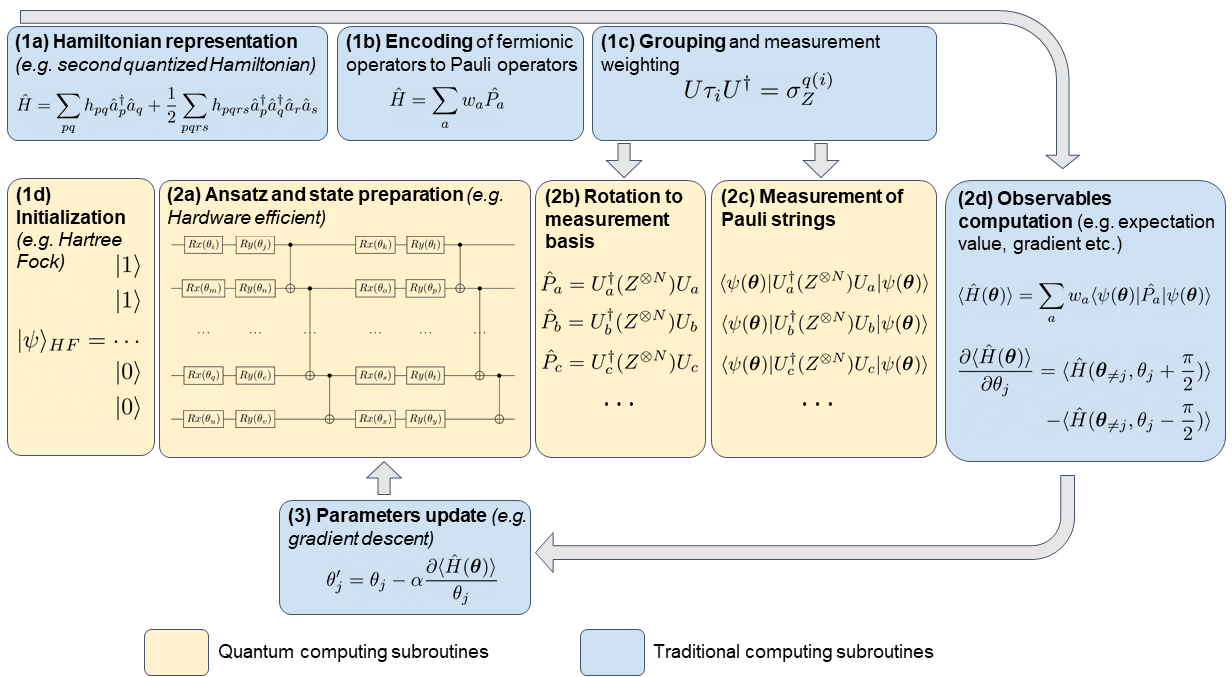
\includegraphics[width=1.0\linewidth]{figures/vqe.png}}

\vspace{6mm}
\end{frame}

\begin{frame}[plain,fragile]
\frametitle{Rotations}

To have any flexibility in the
ansatz $\vert \psi\rangle$, we need to allow for a given parametrization. The most
common approach is to employ the so-called rotation operations given by $R_x$, $R_z$ and $R_y$, where we apply chained
operations of rotating around the various axes by $\boldsymbol{\theta} =
(\theta_1,\ldots,\theta_Q)$ of the Bloch sphere and CNOT operations.

Applications of say the $y$-rotation
specifically ensures that our coefficients always remain real, which
often is satisfactory when dealing with many-body systems.
\end{frame}

\begin{frame}[plain,fragile]
\frametitle{Measurements and more}

After the ansatz has been constructed, the Hamiltonian must
be applied. The Hamiltonian must be written in terms of
Pauli strings in order to perform measurements properly.

To obtain the expectation value
of the ground state energy, one can measure the expectation value of
each Pauli string, 
\begin{align*}
    E(\boldsymbol{\theta}) = \sum_i w_i\langle \psi(\boldsymbol{\theta})\vert P_i \vert \psi(\boldsymbol{\theta})\rangle \equiv \sum_i w_i f_i,
\end{align*}
where $f_i$ is the expectation value of the Pauli string $i$.
\end{frame}

\begin{frame}[plain,fragile]
\frametitle{Collecting data}

This is estimated statistically by considering measurements in the
appropriate basis of the operator in the Pauli string.

With $N_0$ and $N_1$ as the number of $0$ and $1$ measurements respectively, we can estimate $f_i$ since 
\begin{align*}
    f_i = \lim_{N \to \infty} \frac{N_0 - N_1}{N},
\end{align*}
where $N$ as the number of shots (measurements).

Each Pauli string requires its own circuit, where multiple measurements
of each string is required. Adding the results together with the
corresponding weights, the ground state energy can be estimated. To
optimize with respect to  $\boldsymbol{\theta}$, a classical optimizer is often
applied.
\end{frame}

\begin{frame}[plain,fragile]
\frametitle{Ansatzes}

Every possible qubit wavefunction $\left| \psi \right\rangle$ can be presented as a vector: 
\[
\left| \psi \right\rangle = \begin{bmatrix}
\cos{\left( \theta/2 \right)}\\
e^{i \varphi} \cdot \sin{\left( \theta/2 \right)}
\end{bmatrix},
\]

where the numbers $\theta$ and $\varphi$ define a point on the unit
three-dimensional sphere, the so-called  Bloch sphere.

For a random one qubit Hamiltonian, a \emph{good} quantum state preparation
circuit should be able to generate all possible states on the Bloch
sphere.
\end{frame}

\begin{frame}[plain,fragile]
\frametitle{Preparing the states}

Before quantum state preparation, our qubit is in the $\vert 0\rangle$ state.
This corresponds to the vertical position of
the vector in the Bloch sphere. In order to generate any possible
$\left| \psi \right\rangle$ we will apply $R_x(t_1)$ and $R_y(t_2)$
gates on the $\left| 0 \right\rangle$ initial state
\[
R_y(\phi)R_x(\theta) \left| 0 \right\rangle = \left| \psi\right\rangle.
\]

The rotation $R_x(\theta)$
corresponds to the rotation in the Bloch
sphere around the $x$-axis and $R_y(\phi)$ the rotation around the $y$-axis.
\end{frame}

\begin{frame}[plain,fragile]
\frametitle{Rotations used}

These two gates with there parameters ($\theta$ and $\phi$) will generate
for us the trial (ansatz) wavefunctions. The two parameters will be in
control of the Classical Computer and its optimization model.
\end{frame}

\begin{frame}[plain,fragile]
\frametitle{Implementing using qiskit}

\begin{minted}[fontsize=\fontsize{9pt}{9pt},linenos=false,mathescape,baselinestretch=1.0,fontfamily=tt,xleftmargin=2mm]{python}
import numpy as np
from random import random
from qiskit import *
def quantum_state_preparation(circuit, parameters):
    q = circuit.qregs[0] # q is the quantum register where the info about qubits is stored
    circuit.rx(parameters[0], q[0]) # q[0] is our one and only qubit XD
    circuit.ry(parameters[1], q[0])
    return circuit

\end{minted}
\end{frame}

\begin{frame}[plain,fragile]
\frametitle{Expectation values}

To execute the second step of VQE, we need to understand how
expectation values of operators can be estimated via quantum computers
by post-processing measurements of quantum circuits in different
basis sets. To rotate bases, one uses the basis rotator $R_\sigma$ which is
defined for each Pauli gate $\sigma$ to be (using the Hadamard rotation $H$ and Phase rotation $S$)
for a Pauli-$\bm{X}$ matrix
\[
\bm{X}=\bm{R}_{\sigma}\bm{Z}\bm{R}_{\sigma} = \bm{HZH}
\]
for a Pauli-$\bm{Y}$ matrix
\[
\bm{Y}=\bm{R}_{\sigma}\bm{Z}\bm{R}_{\sigma}=\bm{HS}^{\dagger}\bm{ZHS},
\]
and
\[
\bm{Z}=\bm{R}_{\sigma}\bm{Z}\bm{R}_{\sigma}=\bm{I}\bm{Z}\bm{I}=\bm{Z}.
\]
\end{frame}

\begin{frame}[plain,fragile]
\frametitle{Measurements of eigenvalues of the Pauli operators}

We can show that these rotations allow us to measure the eigenvalues of the Pauli operators. The eigenvectors of the Pauli $\bm{X}$ gate are
\[
\vert\pm\rangle = \frac{\vert 0\rangle \pm \vert 1\rangle}{\sqrt{2}},
\]
with eigenvalues $\pm 1$.
Acting on the eigenstates with the rotation gives
\[
\bm{H}\vert +\rangle = +1\vert 0\rangle,
\]
and
\[
\bm{H}\vert -\rangle = -1\vert 1\rangle.
\]
\end{frame}

\begin{frame}[plain,fragile]
\frametitle{Single-qubit states}

Any single-qubit state can be written as a linear combination of these eigenvectors,
\[
\vert \psi\rangle = \alpha \vert +\rangle + \beta \vert -\rangle.
\]
We then have the following expectation value for the Pauli $\bm{X}$ operator
\[
\langle \vert X\vert \rangle = \langle \psi\vert X \vert \psi\rangle = |\alpha|^2 - |\beta|^2.
\]
However, we can only measure the qubits in the computational basis. Applying the rotation to our state gives
\[
H \vert \psi\rangle = \alpha \vert 0\rangle - \beta \vert 1\rangle.
\]
\end{frame}

\begin{frame}[plain,fragile]
\frametitle{Measurements and computational basis}

We have seen how to rewrite the above sinple $2\times 2$ eiegenvalue problem in terms of a Hamiltonian defined by Pauli $\bm{X}$ and $\bm{Z}$ matrices,
and the identity matrix $\bm{I}$.
Let us make this Hamiltonian that involves only one qubit somewhat more general
\[
\left\langle \psi \right| \mathcal{H} \left| \psi \right\rangle = a \cdot \left\langle \psi \right| \bm{I} \left| \psi \right\rangle + b \cdot \left\langle \psi \right| \bm{Z} \left| \psi \right\rangle + c \cdot \left\langle \psi \right| \bm{X} \left| \psi \right\rangle + d \cdot \left\langle \psi \right| \bm{Y} \left| \psi \right\rangle.
\]
\end{frame}

\begin{frame}[plain,fragile]
\frametitle{Expectation value of $\bm{I}$}

For the $I$ operator the expectation value is always unity:

\[
\left\langle \psi \right| \bm{I} \left| \psi \right\rangle = 1.
\]
Its contribution to the overall expectaction value is thus given by the constant $a$.
\end{frame}

\begin{frame}[plain,fragile]
\frametitle{The Pauli matrices}

For the rest of the Pauli operators, we make the following remark:
every one qubit quantum state $\left| \psi \right\rangle$ can be
represented via different sets of basis vectors:

\[
\left| \psi \right\rangle = c_1^z \cdot \left| 0 \right\rangle + c_2^z \cdot \left| 1 \right\rangle = c_1^x \cdot \left| + \right\rangle + c_2^x \cdot \left| - \right\rangle = c_1^y \cdot \left| +i \right\rangle + c_2^y \cdot \left| -i \right\rangle.
\]
\end{frame}

\begin{frame}[plain,fragile]
\frametitle{In more detail}

We have
\begin{align*}
&\text{Z-eigenvectors} \qquad
\left| 0 \right\rangle = \begin{bmatrix}
1\\
0
\end{bmatrix},
&&\left| 1 \right\rangle = \begin{bmatrix}
0\\
1
\end{bmatrix},
\end{align*}
\end{frame}

\begin{frame}[plain,fragile]
\frametitle{For the other two matrices}

\begin{align*}
&\text{X-eigenvectors} \qquad
\left| + \right\rangle = \frac{1}{\sqrt{2}} \begin{bmatrix}
1\\
1
\end{bmatrix},
&&\left| - \right\rangle = \frac{1}{\sqrt{2}} \begin{bmatrix}
1\\
-1
\end{bmatrix},
\\
&\text{Y-eigenvectors} \qquad
\left| +i \right\rangle = \frac{1}{\sqrt{2}} \begin{bmatrix}
1\\
i
\end{bmatrix}, 
&&\left| -i \right\rangle = \frac{1}{\sqrt{2}} \begin{bmatrix}
1\\
-i
\end{bmatrix}.
\end{align*}
\end{frame}

\begin{frame}[plain,fragile]
\frametitle{Analyzing these equations}

The first presented eigenvectors for each Pauli operator have eigenvalues equal to $+1$: $Z \left| 0 \right\rangle = +1\left| 0 \right\rangle$, $X \left| + \right\rangle = +1\left| + \right\rangle$, $Y \left| +i \right\rangle = +1\left| +i \right\rangle$, respectively.

The second eigenvectors for each Pauli operator have eigenvalues equal to $-1$: $Z \left| 1 \right\rangle = -1\left| 1 \right\rangle$, $X \left| - \right\rangle = -1\left| - \right\rangle$, $Y \left| -i \right\rangle = -1\left| -i \right\rangle$, respectively
\end{frame}

\begin{frame}[plain,fragile]
\frametitle{Explicit eigenvalues}

Now, let us calculate the expectation values of these Pauli operators: 

\begin{align*}
\left\langle \psi \right| \bm{Z} \left| \psi \right\rangle &= \left( {c_1^z}^* \cdot \left\langle 0 \right| + {c_2^z}^* \cdot \left\langle 1 \right| \right) Z \left( c_1^z \cdot \left| 0 \right\rangle + c_2^z \cdot \left| 1 \right\rangle \right) = {\left| c_1^z \right|}^2 - {\left| c_2^z \right|}^2,
\\
\left\langle \psi \right| \bm{X} \left| \psi \right\rangle &= \left( {c_1^x}^* \cdot \left\langle + \right| + {c_2^x}^* \cdot \left\langle - \right| \right) X \left( c_1^x \cdot \left| + \right\rangle + c_2^x \cdot \left| - \right\rangle \right) = {\left| c_1^x \right|}^2 - {\left| c_2^x \right|}^2,
\\
\left\langle \psi \right| \bm{Y} \left| \psi \right\rangle &= \left( {c_1^y}^* \cdot \left\langle +i \right| + {c_2^y}^* \cdot \left\langle -i \right| \right) Y \left( c_1^y \cdot \left| +i \right\rangle + c_2^y \cdot \left| -i \right\rangle \right) = {\left| c_1^y \right|}^2 - {\left| c_2^y \right|}^2.
\end{align*}
\end{frame}

\begin{frame}[plain,fragile]
\frametitle{Computational basis}

The above equations require that we can make measurements in the chosen basis sets.

However, this may not be possible. The difficulty comes  from the fact that one may have the possibility
to measure only in the $\bm{Z}$-basis. To solve this difficulty we still do
a $\bm{Z}$-basis measurement, but, before that, we apply specific operators
to the $\left| \psi \right\rangle$ state.
\end{frame}

\begin{frame}[plain,fragile]
\frametitle{Unitary transformation of $\bm{X}$}

If we use the Hadamard gate
\[
\bm{H} = \frac{1}{\sqrt{2}}\begin{bmatrix}
1 & 1\\
1 & -1
\end{bmatrix},
\]
we can rewrite
\[
\bm{X}=\bm{HZH}.
\]

The Hadamard gate/matrix is a unitary matrix with the property that $\bm{H}^2=\bm{I}$.
\end{frame}

\begin{frame}[plain,fragile]
\frametitle{Generalizing}

For the one-qubit Hamiltonian we have toyed with till now, we can thus
rewrite in an easy way the Hamiltonian so that we can perform
measurements using our favorite computational basis.

The transformation of the Pauli-$\bm{X}$ matrix can be generalized, as
we will see in more detail below for the two-qubit Hamiltonian and next week for 
the Lipkin model, to the following expression
\[
\mathcal{P}=\bm{U}^{\dagger}\bm{M}\bm{U},
\]
where $\mathcal{P}$ represents some combination of the Pauli matrices and
the identity matrix, $\bm{U}$ is a unitary matrix and $\bm{M}$
represents the gate/matrix which performs the measurements, often
represented by a Pauli-$\bm{Z}$ gate/matrix.
\end{frame}

\begin{frame}[plain,fragile]
\frametitle{Interpretations}

This tells us that we are able to estimate $|\alpha|^2$ and
$|\beta|^2$ (and hence the expectation value of the Pauli $\bm{X}$
operator) by using a rotation and measure the
resulting state in the computational basis. We can show this for the
Pauli $\bm{Z}$ and Pauli $\bm{Y}$ similarly.
\end{frame}

\begin{frame}[plain,fragile]
\frametitle{Reminder on rotations}

Note the following identity of the basis rotator
\[
\bm{R}^\dagger_\sigma \bm{Z} \bm{R}_\sigma = \bm{\sigma,}
\]
which follows from the fact that $\bm{HZH}=\bm{X}$ and $\bm{SXS}^\dagger=\bm{Y}$.
\end{frame}

\begin{frame}[plain,fragile]
\frametitle{Why do we measure on one qubit? First consideration}

In quantum computing, measurements are typically performed on one
qubit at a time due to a combination of theoretical, practical, and
algorithmic considerations:

\begin{block}{Algorithmic Requirements: }
\begin{enumerate}
\item Adaptive Processing: Many quantum algorithms, such as quantum teleportation or error correction, require mid-circuit measurements. The outcomes determine subsequent operations, necessitating sequential measurements to adapt the circuit dynamically.

\item Partial Information Extraction: Algorithms often need only specific qubits' results (e.g., in Shor's algorithm), making full-system measurements unnecessary.
\end{enumerate}

\noindent
\end{block}
\end{frame}

\begin{frame}[plain,fragile]
\frametitle{Why do we measure on one qubit? Second consideration}

\begin{block}{Quantum Mechanical Principles: }
\begin{enumerate}
\item Collapse and Entanglement: Measuring a qubit collapses its state, potentially affecting entangled qubits. Sequential measurements allow controlled extraction of information while managing entanglement.

\item Measurement Basis: Most algorithms use the computational basis (individual qubit measurements). Joint measurements in entangled bases are possible but require complex setups and are not always needed.
\end{enumerate}

\noindent
\end{block}
\end{frame}

\begin{frame}[plain,fragile]
\frametitle{Why do we measure on one qubit? Third consideration}

\begin{block}{Practical Hardware Limitations: }
\begin{enumerate}
\item Crosstalk and Noise: Simultaneous measurements risk disturbing neighboring qubits due to hardware imperfections, especially in noisy intermediate-scale quantum (NISQ) devices.

\item Readout Constraints: Physical implementations (e.g., superconducting qubits) may have limited readout bandwidth, forcing sequential measurements.
\end{enumerate}

\noindent
\end{block}
\end{frame}

\begin{frame}[plain,fragile]
\frametitle{Why do we measure on one qubit? Fourth consideration}

\begin{block}{Resource Management: }
\begin{enumerate}
\item Qubit Reuse: Ancilla qubits (e.g., in error correction) are measured, reset, and reused, requiring sequential handling to avoid disrupting computational qubits.
\end{enumerate}

\noindent
\end{block}
\begin{block}{Conclusion: }
While joint measurements are theoretically possible, the dominant practice of measuring one qubit at a time stems from algorithmic adaptability, hardware limitations, and the need to minimize quantum state disturbance. This approach balances efficiency, practicality, and the constraints of current quantum systems.
\end{block}
\end{frame}

\begin{frame}[plain,fragile]
\frametitle{Arbitrary Pauli gate}

With this, we see that the expectation value of an arbitrary
Pauli-gate $\sigma$ in the state $\vert\psi\rangle$ can be expressed as a linear combination of probabilities
\begin{align*}
E_{\psi}(\sigma)
&= \langle \psi\vert\sigma\vert\psi\rangle \nonumber \\
&=\langle\psi\vert R_{\sigma}^{\dagger}ZR_{\sigma}\vert\psi\rangle =\langle \phi\vert Z\vert \phi\rangle \nonumber \\
&=\langle\phi\vert\left(\sum_{x\in\{0,1\}}(-1)^x\vert x\rangle\langle x\vert\right)\vert\phi\rangle \nonumber \\
&=\sum_{x\in\{0,1\}}(-1)^x\vert\langle x\vert \phi\rangle\vert^2\nonumber \\
&=\sum_{x\in\{0,1\}}(-1)^xP(\vert \phi\rangle\to\vert x\rangle),
\end{align*}

where $\vert \phi\rangle=\vert R_\sigma\phi\rangle$ and
$P(\vert \phi\rangle\to\vert x\rangle$ is the probability that the state
$\vert \phi\rangle$ collapses to the state $\vert x\rangle$ when measured.
\end{frame}

\begin{frame}[plain,fragile]
\frametitle{Arbitrary string of Pauli operators}

This can
be extended to any arbitrary Pauli string: consider the string of
Pauli operators $P=\bigotimes_{p\in Q}\sigma_p$ which acts
non-trivially on the set of qubits $Q$ which is a subset of the total
set of $n$ qubits in the system. Then

\begin{align*}
E_{\psi}\left(P\right)
&=\langle \psi\vert\left(\bigotimes_{p\in Q}\sigma_p\right)\vert \psi\rangle \nonumber \\
&=\langle \psi\vert\left(\bigotimes_{p\in Q}\sigma_p\right)
\left(\bigotimes_{q\notin Q}I_q\right)\vert \psi\rangle \nonumber \\
&=\langle \psi\vert\left(\bigotimes_{p \in Q}R_{\sigma_p}^{\dagger}Z_pR_{\sigma_p}\right)
\left(\bigotimes_{q\notin Q}I_q\right)\vert \psi\rangle \nonumber \\
&=
\langle \psi\vert\left(\bigotimes_{p \in Q}R_{\sigma_p}^{\dagger}\right)
\left(\bigotimes_{p \in Q}Z_p\right)
\left(\bigotimes_{q\notin Q}I_q\right)
\left(\bigotimes_{p \in Q}R_{\sigma_p}\right)\vert \psi\rangle \nonumber 
\end{align*}
\end{frame}

\begin{frame}[plain,fragile]
\frametitle{This gives us}

\begin{align*}
E_{\psi}\left(P\right)
&=
\langle \phi\vert
\left(\bigotimes_{p \in Q}Z_p\right)
\left(\bigotimes_{q\notin Q}I_q\right)
\vert \phi\rangle \nonumber \\
&=
\langle \phi\vert
\left(\bigotimes_{p\in Q}\sum_{x_p\in\{0_p,1_p\}}(-1)^{x_p}\vert x_p\rangle\langle x_p\vert\right)
\left(\bigotimes_{q\notin Q}\sum_{y_q\in\{0_q,1_q\}}\vert y_q\rangle\langle y_q\vert\right)
\vert \phi\rangle 
\nonumber 
\\
&=
\langle \phi\vert
\left(\sum_{x\in\{0,1\}^n}(-1)^{\sum_{p\in Q}x_p}\vert x\rangle\langle x\vert\right)
\vert \phi\rangle 
\nonumber 
\\
&=
\sum_{x\in\{0,1\}^n}(-1)^{\sum_{p\in Q}x_p}\vert\langle x\vert\vert \phi\rangle\vert^2
\nonumber 
\\
&=
\sum_{x\in\{0,1\}^n}(-1)^{\sum_{p\in Q}x_p}P(\vert \phi\rangle\to\vert x\rangle),
\end{align*}
where $\vert \phi\rangle=\vert \bigotimes_{p\in Q}R_{\sigma_p}\psi\rangle$.
\end{frame}

\begin{frame}[plain,fragile]
\frametitle{Final observables}

Finally, because the expectation value is
linear
\[
E_\psi\left(\sum_{m}\lambda_mP_m\right) = \sum_m\lambda_mE_\psi(P_m),
\]
one can estimate any observable that can be written as a linear combination of Pauli-string terms.
\end{frame}

\begin{frame}[plain,fragile]
\frametitle{Measurement}

To estimate the probability $P(\vert \phi\rangle\to \vert x\rangle)$ from the
previous results, one prepares the state $\vert \phi\rangle$ on a quantum
computer and measures it, and then repeats this process (prepare and
measure) several times. The probability $P(\vert \phi\rangle\to \vert x\rangle)$ is
estimated to be the number of times that one measures the bit-string
$x$ divided by the total number of measurements that one makes; that
is

\[
P(\vert \phi\rangle\to \vert x\rangle\rangle \approx \sum_{m=1}^M\frac{x_m}{M},
\]
where $x_m=1$
if the result of measurement is $x$ and  $0$ if the result of measurement is not $x$.
\end{frame}

\begin{frame}[plain,fragile]
\frametitle{\href{{https://en.wikipedia.org/wiki/Law_of_large_numbers}}{Law of large numbers} aka Bernoulli's theorem}

By the law of large numbers the approximation approaches equality as
$M$ goes to infinity

\[
P(\vert \phi\rangle\to \vert x\rangle) = \lim_{M\to\infty}\sum_{m=1}^M\frac{x_m}{M}.
\]

As we obviously do not have infinite time nor infinite quantum
computers (which could be run in parallel), we must truncate our
number of measurement $M$ to a finite, but sufficiently large
number. More precisely, for precision $\epsilon$, each expectation
estimation subroutine within VQE requires $\mathcal{O}(1/\epsilon^2)$
samples from circuits with depth $\mathcal{O}(1)$.
\end{frame}

\end{document}
